\chapter{Compiler optimizations: behaviour, effects and recommendations}
\label{ch:optimizations}

\section{Introduction}
Compiler optimizations change generated instruction sequences, code size, and runtime behaviour in ways that can be decisive for correctness and observability on custom processors. This chapter examines the impact of standard GCC optimization levels on the RWU-RV64I core and the verification workflow developed in this project. We document experiments performed with three representative C workloads, analyse root causes for observed pass/fail behaviour in the simulation testbench, and provide concrete recommendations for the RWU-RV64I toolchain and verification flow. The experiments support reproducibility by using the same linker script and startup code described in Chapter~\ref{ch:toolchain} and the simulation/testbench harness described in Chapter~\ref{ch:eclipse}.

\section{Goals and Scope}

This chapter pursues three primary objectives:
\begin{enumerate}
  \item To quantify the impact of different compiler optimization levels on binary code size and observable program behavior.
  \item To identify and analyze the causes of build-time failures and simulation mismatches encountered during compilation and execution.
  \item To propose recommendations for establishing a stable development workflow that balances debuggability, correctness, and binary size efficiency.
\end{enumerate}

The scope of this study is intentionally practical.  
All experiments are conducted using a minimal, freestanding GNU RISC-V toolchain (\texttt{riscv64-unknown-elf-gcc}) configured with the following options:
\begin{quote}
\texttt{-march=rv64i -mabi=lp64 -ffreestanding -nostdlib -msmall-data-limit=0}
\end{quote}

The same linker script and startup files described in earlier chapters are reused to ensure consistency across builds.  
The three C test programs employed for this evaluation are included in Appendix~\ref{app:optimization-programs}.



\section{Experimental setup}
\label{sec:optim-setup}

\subsection{Toolchain and build commands}
All experiments used the same RISC-V cross-compiler and the same build infrastructure. Example compiler and link commands (extracted from the build logs) are:

\begin{verbatim}
riscv64-unknown-elf-gcc -march=rv64i -mabi=lp64 -ffreestanding\
 -nostdlib -msmall-data-limit=0 -I -O2 -g -c program.c -o program.o

riscv64-unknown-elf-gcc -march=rv64i -mabi=lp64 -ffreestanding \
 -nostdlib -T linker.ld -Wl,-Map="test.map" -o test.elf test.o crt0.o
\end{verbatim}

Each experiment varied only the optimization flag among: \texttt{-O0},  \texttt{-O1}, \texttt{-O2}, \texttt{-O3}, \texttt{-Os}, \texttt{-Ofast}.

\subsection{Runtime and verification infrastructure}
The verification flow employs the following components:
\begin{itemize}
  \item A SystemVerilog simulation testbench that drives the RWU-RV64I core and monitors GPIO outputs emitted through the lightweight \texttt{rwu\_print} mechanism (the same testbench described in Chapter~\ref{ch:eclipse}).
  
  \item A DMEM inspection utility (\texttt{rwu\_store64}) that writes a 64-bit marker to a known data memory location, enabling offline verification by the testbench.
  
  \item The generated Verilog memory files (\texttt{*.mem}) produced by the command:
  \begin{quote}
    \texttt{riscv64-unknown-elf-objcopy -O verilog}
  \end{quote}
  These files are then loaded into the simulator memory image for execution.
\end{itemize}


\subsection{Programs under test}
The three test programs exercise different optimization-sensitive patterns:
\begin{enumerate}
  \item \textbf{opt\_workload.c}: multi-part workload with many small functions, a tight arithmetic loop, a 16-case switch, and a small memcpy-like routine. Emits labeled GPIO markers E0..E5 and stores a 64-bit DMEM marker.
  \item \textbf{square test (test.c)}: small arithmetic function that computes a square inside a loop and prints markers.
  \item \textbf{test\_simple\_gpio.c}: simple arithmetic sequence with predictable GPIO outputs (intended to exercise constant-folding, arithmetic, and small-control flow).
\end{enumerate}

The exact program listings are placed in Appendix~\ref{app:optimization-programs}.

\subsection{Measurements}
For each program and optimization level we recorded:
\begin{itemize}
  \item Build success / failure (linker errors).
  \item The \texttt{.text}, \texttt{.data} and \texttt{.bss} sizes from \texttt{size}.
  \item Simulation outcome (which GPIO markers were observed; pass/fail).
  \item The produced \texttt{.mem} image (retained for offline comparison).
\end{itemize}

\section{Results}
\label{sec:optim-results}

Tables~\ref{tab:opt-workload}, \ref{tab:square-test} and \ref{tab:simple-gpio} summarise the results extracted from the build logs and simulation runs.

\begin{table}[htbp]
  \centering
  \caption{\texttt{opt\_workload.c}: Code size and simulation outcome vs. optimization level}
  \label{tab:opt-workload}
  \begin{tabularx}{\textwidth}{@{} l c c c c >{\raggedright\arraybackslash}X @{}}
    \toprule
    \textbf{Optimization}
      & \textbf{\texttt{.text} (bytes)}
      & \textbf{\texttt{.data}}
      & \textbf{\texttt{.bss}}
      & \textbf{Build}
      & \textbf{Simulation} \\
    \midrule
    \texttt{-O0}           & 1920 & 0 & 136 & OK & Failed (did not run) \\
    \texttt{-O}/\texttt{-O1} & 712  & 0 & 136 & OK &Failed (reached marker E3) \\
    \texttt{-O2}           & 472  & 0 & 136 & OK & All tests cases passed \\
    \texttt{-O3}           & 440  & 0 & 72  & OK & All tests cases passed \\
    \texttt{-Os}           & 480  & 0 & 136 & OK & All tests cases passed \\
    \texttt{-Ofast}        & 440  & 0 & 72  & OK & All tests cases passed \\
    \bottomrule
  \end{tabularx}
\end{table}


\begin{table}[htbp]
  \centering
  \caption{Square test (\texttt{test.c}): code size and outcome vs. optimization level}
  \label{tab:square-test}
  \begin{tabularx}{\textwidth}{@{} l c c c c >{\raggedright\arraybackslash}X @{}}
    \toprule
    \textbf{Optimization}
      & \textbf{\texttt{.text} (bytes)}
      & \textbf{\texttt{.data}}
      & \textbf{\texttt{.bss}}
      & \textbf{Build}
      & \textbf{Simulation} \\
    \midrule
    \texttt{-O0}            & --- & --- & --- & Failed &               Failed \\
    \texttt{-O}/\texttt{-O1} & 140 & 0   & 0   & OK                    & All test cases passed. \\
    \texttt{-O2}            & 140 & 0   & 0   & OK                    & All test cases passed. \\
    \texttt{-O3}            & 140 & 0   & 0   & OK                    & All test cases passed. \\
    \texttt{-Os}            & 136 & 0   & 0   & OK                    & All test cases passed. \\
    \texttt{-Ofast}         & 140 & 0   & 0   & OK                    & All test cases passed. \\
    \bottomrule
  \end{tabularx}
\end{table}

\begin{table}[htbp]
  \centering
  \caption{test\_simple\_gpio.c: code size and outcome vs. optimization level}
  \label{tab:simple-gpio}
  \begin{tabularx}{\textwidth}{@{} l c c c c >{\raggedright\arraybackslash}X @{}}
    \toprule
    \textbf{Optimization}
      & \textbf{\texttt{.text} (bytes)}
      & \textbf{\texttt{.data}}
      & \textbf{\texttt{.bss}}
      & \textbf{Build}
      & \textbf{Simulation} \\
    \midrule
    \texttt{-O0}            & 336 & 0 & 8   & OK & No test cases passed (failed). \\
    \texttt{-O}/\texttt{-O1} & 108 & 0 & 0   & OK & All test cases passed. \\
    \texttt{-O2}            & 108 & 0 & 0   & OK & All test cases passed. \\
    \texttt{-O3}            & 108 & 0 & 0   & OK & All test cases passed. \\
    \texttt{-Os}            & 104 & 0 & 0   & OK & All test cases passed. \\
    \texttt{-Ofast}         & 108 & 0 & 0   & OK & All test cases passed. \\
    \bottomrule
  \end{tabularx}
\end{table}

\noindent In summary:
\begin{itemize}
  \item Optimized images (\texttt{-O2}, \texttt{-O3}, \texttt{-Os}, \texttt{-Ofast}) were consistently smaller and passed the simulation validation for all three workloads.
  \item Unoptimized builds (\texttt{-O0}) either failed at link time (square test) or produced images that the testbench rejected (opt\_workload and test\_simple\_gpio).
  \item Intermediate optimization (\texttt{-O}/\texttt{-O1}) sometimes improved results but was not as robust for the complex workload as \texttt{-O2} and above.
\end{itemize}

\section{Analysis: root causes and mechanisms}
This section explains the observed behaviour and links it to specific compiler transformations.

\subsection{Compiler helper calls and freestanding builds}
The linker error observed for the square test at \texttt{-O0} (\texttt{undefined reference to \_\_muldi3}) shows that, at low optimization, GCC can emit calls to libgcc helper routines (for example, for multi-word arithmetic) which are not available in a minimal freestanding environment when \texttt{-nostdlib} is used. At higher optimization levels the compiler often transforms or replaces such operations with inline code that does not require external helpers, which explains why the problem disappears for \texttt{-O1} and above.

\subsection{Inlining, dead-code elimination and code density}
The large reduction in \texttt{.text} size for \texttt{opt\_workload.c} (from 1920 bytes at \texttt{-O0} to 440--480 bytes at \texttt{-O2}/\texttt{-O3}/\texttt{-Os}) is primarily explained by inlining of frequently-called small functions, removal of redundant temporaries, and dead-code elimination. In practice this means:
\begin{itemize}
  \item Function call overhead disappears and is replaced with tighter sequences of arithmetic and logical instructions.
  \item The number of branch instructions and memory accesses decreases, which changes the timing and ordering of observable I/O (GPIO writes).
\end{itemize}

\subsection{Loop optimizations and strength reduction}
The \texttt{loop\_heavy} function benefits from standard loop optimizations at higher optimization levels (induction variable simplification, strength reduction, unrolling when profitable). Those optimizations reduce instruction counts and may eliminate index computations that would otherwise interact with DMEM or cause additional side effects.

\subsection{Switch-case codegen: branch chain vs jump table}
Compilers may implement `switch` statements either as a chain of conditional branches, or as a jump table. At high optimization levels and for dense case ranges the compiler typically emits a compact jump table. This reduces code size and branch mispredictions (in real hardware) and also simplifies the sequence of instructions executed in the simulator, improving the likelihood the TB observes the expected GPIO sequence.

\subsection{Testbench observability and timing sensitivity}
The verification TB in this project samples GPIO writes and validates an expected marker sequence (E0..E5) and DMEM sentinel. Because compiler optimizations can reorder or remove intermediary operations, the exact timing or presence of transient GPIO writes at \texttt{-O0} differs from optimized builds. The TB therefore may register mismatches even if the logical computation is correct, simply because the TB is sensitive to instruction-level timing and the unoptimized image produces additional/interleaved events.



\section{Experimental verification and hardware output}
\label{sec:optim-verify}

To confirm the functional correctness of the RWU-RV64I toolchain and verify that compiler optimizations preserve expected behaviour, a conditional test program was implemented, compiled, simulated, and executed on the Zybo Zynq--7000 FPGA board.  
The test validates arithmetic, comparison, and branching instructions, and demonstrates observable GPIO output as a visible indicator of processor execution.

\subsection{Purpose of the test}
The goal of this test is to verify that:
\begin{itemize}
  \item The RWU-RV64I core correctly executes arithmetic and comparison operations.
  \item Conditional branching behaves as intended in optimized binaries.
  \item The GPIO output produced by the \texttt{rwu\_print()} function correctly reflects program logic both in simulation and on physical hardware.
\end{itemize}

To achieve this, a simple C program (Listing~\ref{lst:cond-prog}) was created, where the result of an arithmetic comparison determines which LED pattern is displayed on the Zybo board.

\subsection{Conditional test program}
\begin{lstlisting}[language=C, caption={Conditional LED control program for RWU-RV64I verification.}, label={lst:cond-prog}]
#include "rwu-rv64i.h"

uint64_t a;
const uint64_t b = 5;

int main(void) {
    rwu_dmem_reset();
    uint64_t c = 10;
    uint64_t d = 20;
    a = 20;

    while (1) {
        if ((a + c) > (b + d)) {
            rwu_print(0x0F);  // Turn all LEDs ON
        } else {
            rwu_print(0x03);  // Turn first two LEDs ON
        }
    }
}
\end{lstlisting}

\noindent
The program begins by initializing four variables:  
\texttt{a} (global, writable), \texttt{b} (constant), and two local variables \texttt{c} and \texttt{d}.  
The statement \texttt{rwu\_dmem\_reset()} clears data memory to ensure deterministic results before execution.

Inside the infinite loop, the processor continuously evaluates the condition:
\[
(a + c) > (b + d)
\]
Substituting the initialized values:
\[
(20 + 10) > (5 + 20) \Rightarrow 30 > 25
\]
The condition is true, so the program calls \texttt{rwu\_print(0x0F)}, which sets the lower four GPIO pins high—turning ON all four LEDs on the Zybo board.  
If the condition were false, it would instead call \texttt{rwu\_print(0x03)} to illuminate only the first two LEDs.

Thus, this simple logic simultaneously validates the correctness of arithmetic addition, comparison, and branch instruction handling within the RWU-RV64I processor.

\subsection{Build process confirmation}
The project was built in Eclipse CDT using the \texttt{-O2} optimization flag.  
The cross-compilation produced a valid ELF file, which was converted automatically to Verilog memory and binary images for simulation and FPGA download.  
The complete build console output is shown in Figure~\ref{fig:build-console}, confirming that the build finished with zero errors or warnings.

\begin{figure}[H]
  \centering
  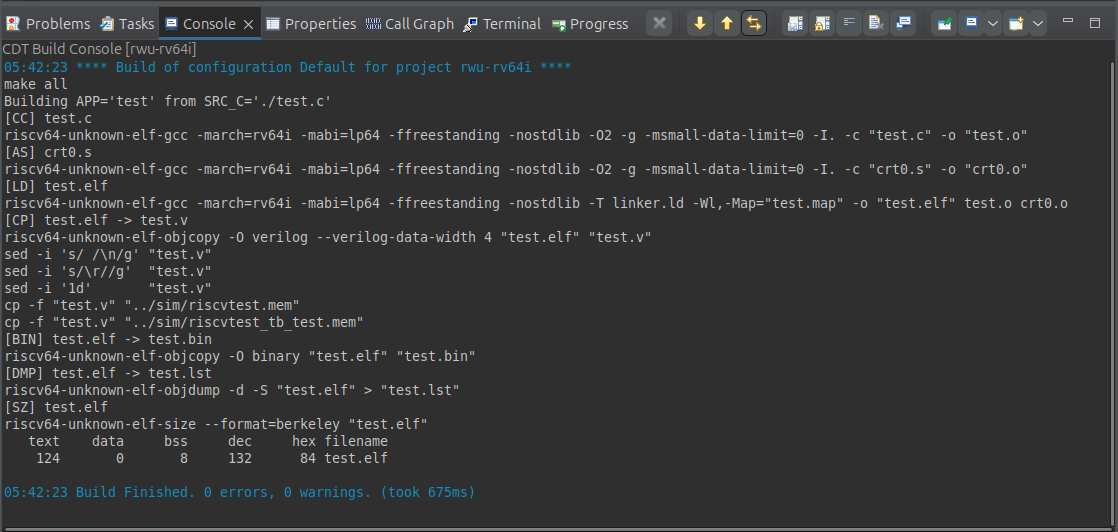
\includegraphics[width=0.95\textwidth]{rwu_output1.png}
  \caption{Successful build of the conditional test program using the RWU-RV64I GCC toolchain in Eclipse CDT.}
  \label{fig:build-console}
\end{figure}

\subsection{Simulation verification in XSIM}
The generated memory image was loaded into the Vivado XSIM testbench.  
Figure~\ref{fig:sim-console} shows the XSIM console output.  
The simulation log reports the message:
\texttt{A+C is greater than B+D 0xF} followed by \texttt{Simulation succeeded}, indicating that the conditional branch executed correctly and that the GPIO value \texttt{0x0F} was produced.

\begin{figure}[H]
  \centering
  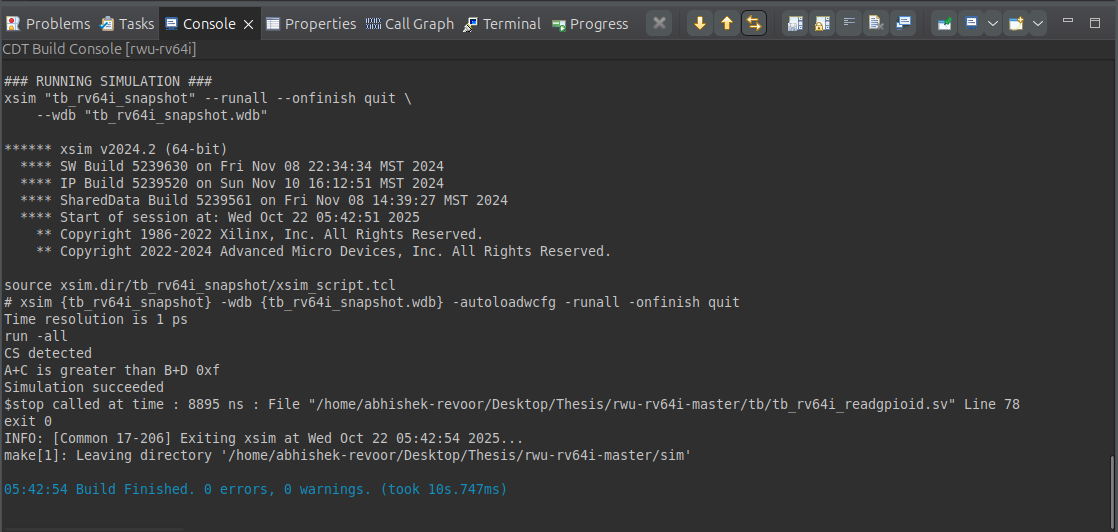
\includegraphics[width=0.95\textwidth]{rwu_output2.png}
  \caption{XSIM simulation console showing correct conditional result and successful program termination.}
  \label{fig:sim-console}
\end{figure}

\subsection{Waveform analysis}
The captured waveform from XSIM is presented in Figure~\ref{fig:sim-wave}.  
The signal \texttt{gpio\_s[7:0]} carries the output value driven by the \texttt{rwu\_print()} function.  
Here, it maintains a stable value of \texttt{0x0F}, verifying that the branch condition evaluated as true (\texttt{30 > 25}).  
This confirms that both arithmetic and logical instructions were correctly synthesized and executed by the RWU-RV64I processor model.

\begin{figure}[H]
  \centering
  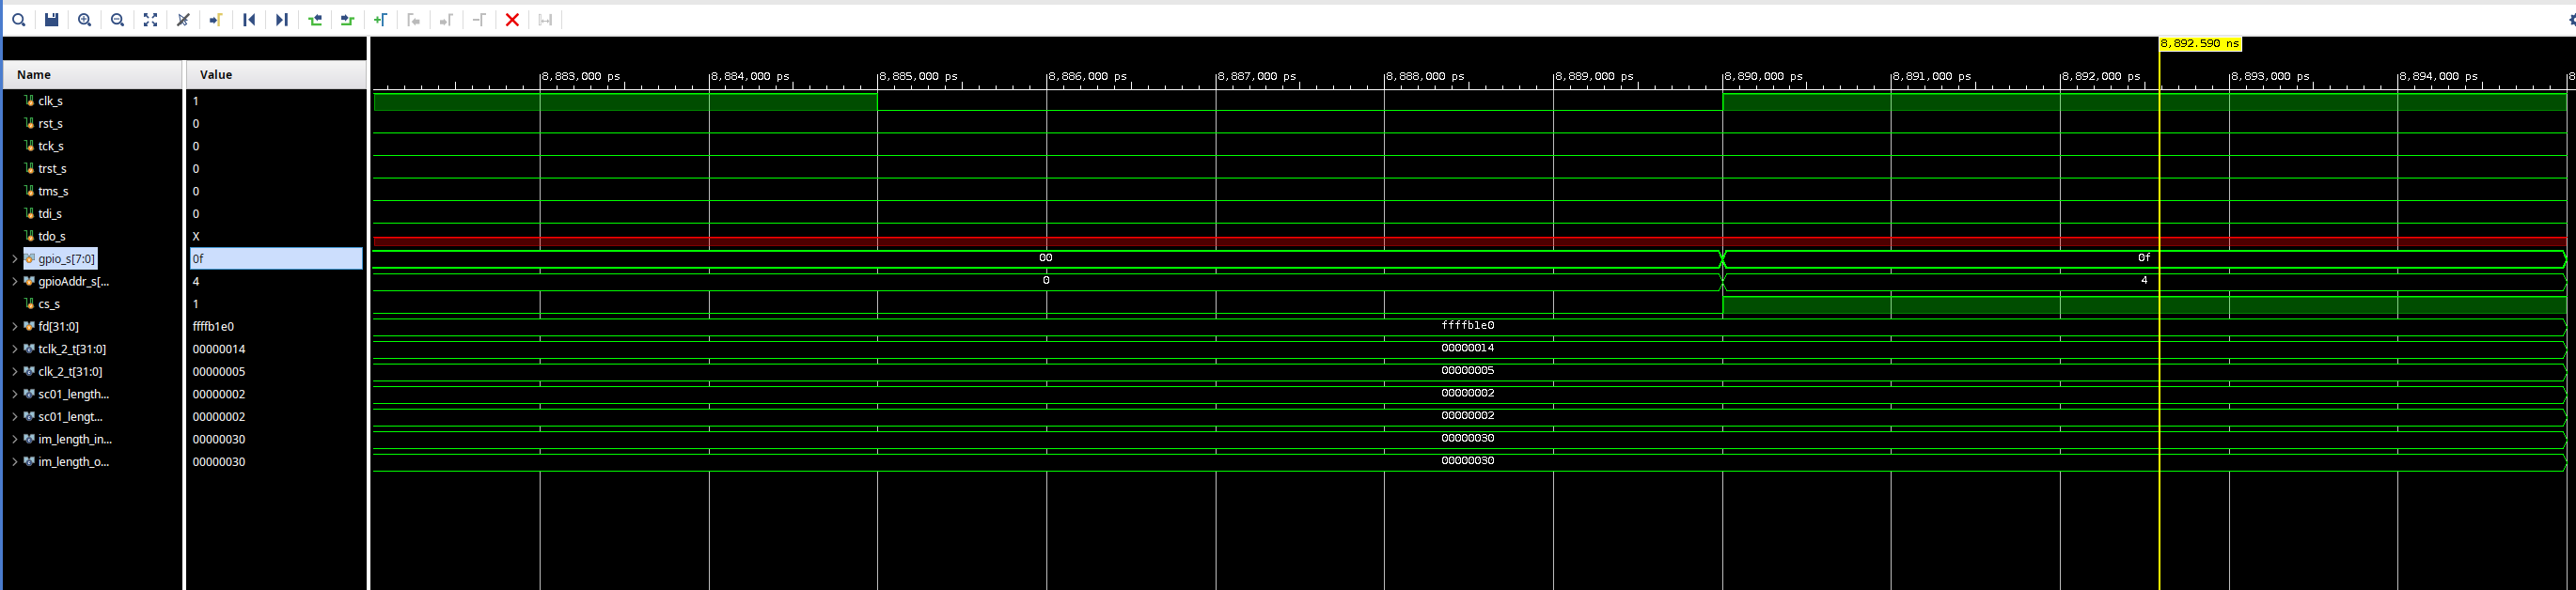
\includegraphics[width=\textwidth]{rwu_output3.png}
  \caption{XSIM waveform showing GPIO output (\texttt{gpio\_s[7:0]} = 0x0F) for the satisfied branch condition.}
  \label{fig:sim-wave}
\end{figure}

\subsection{FPGA hardware execution}
After successful simulation, the generated memory file (\texttt{test.mem}) was programmed into the Zybo FPGA configuration.  
Figure~\ref{fig:fpga-output} shows the physical output on the board, where all four user LEDs are ON.  
This directly corresponds to the logical output value \texttt{GPIO = 0x0F}, confirming that the processor core, memory interface, and GPIO hardware mapping function identically in real hardware.

\begin{figure}[H]
  \centering
  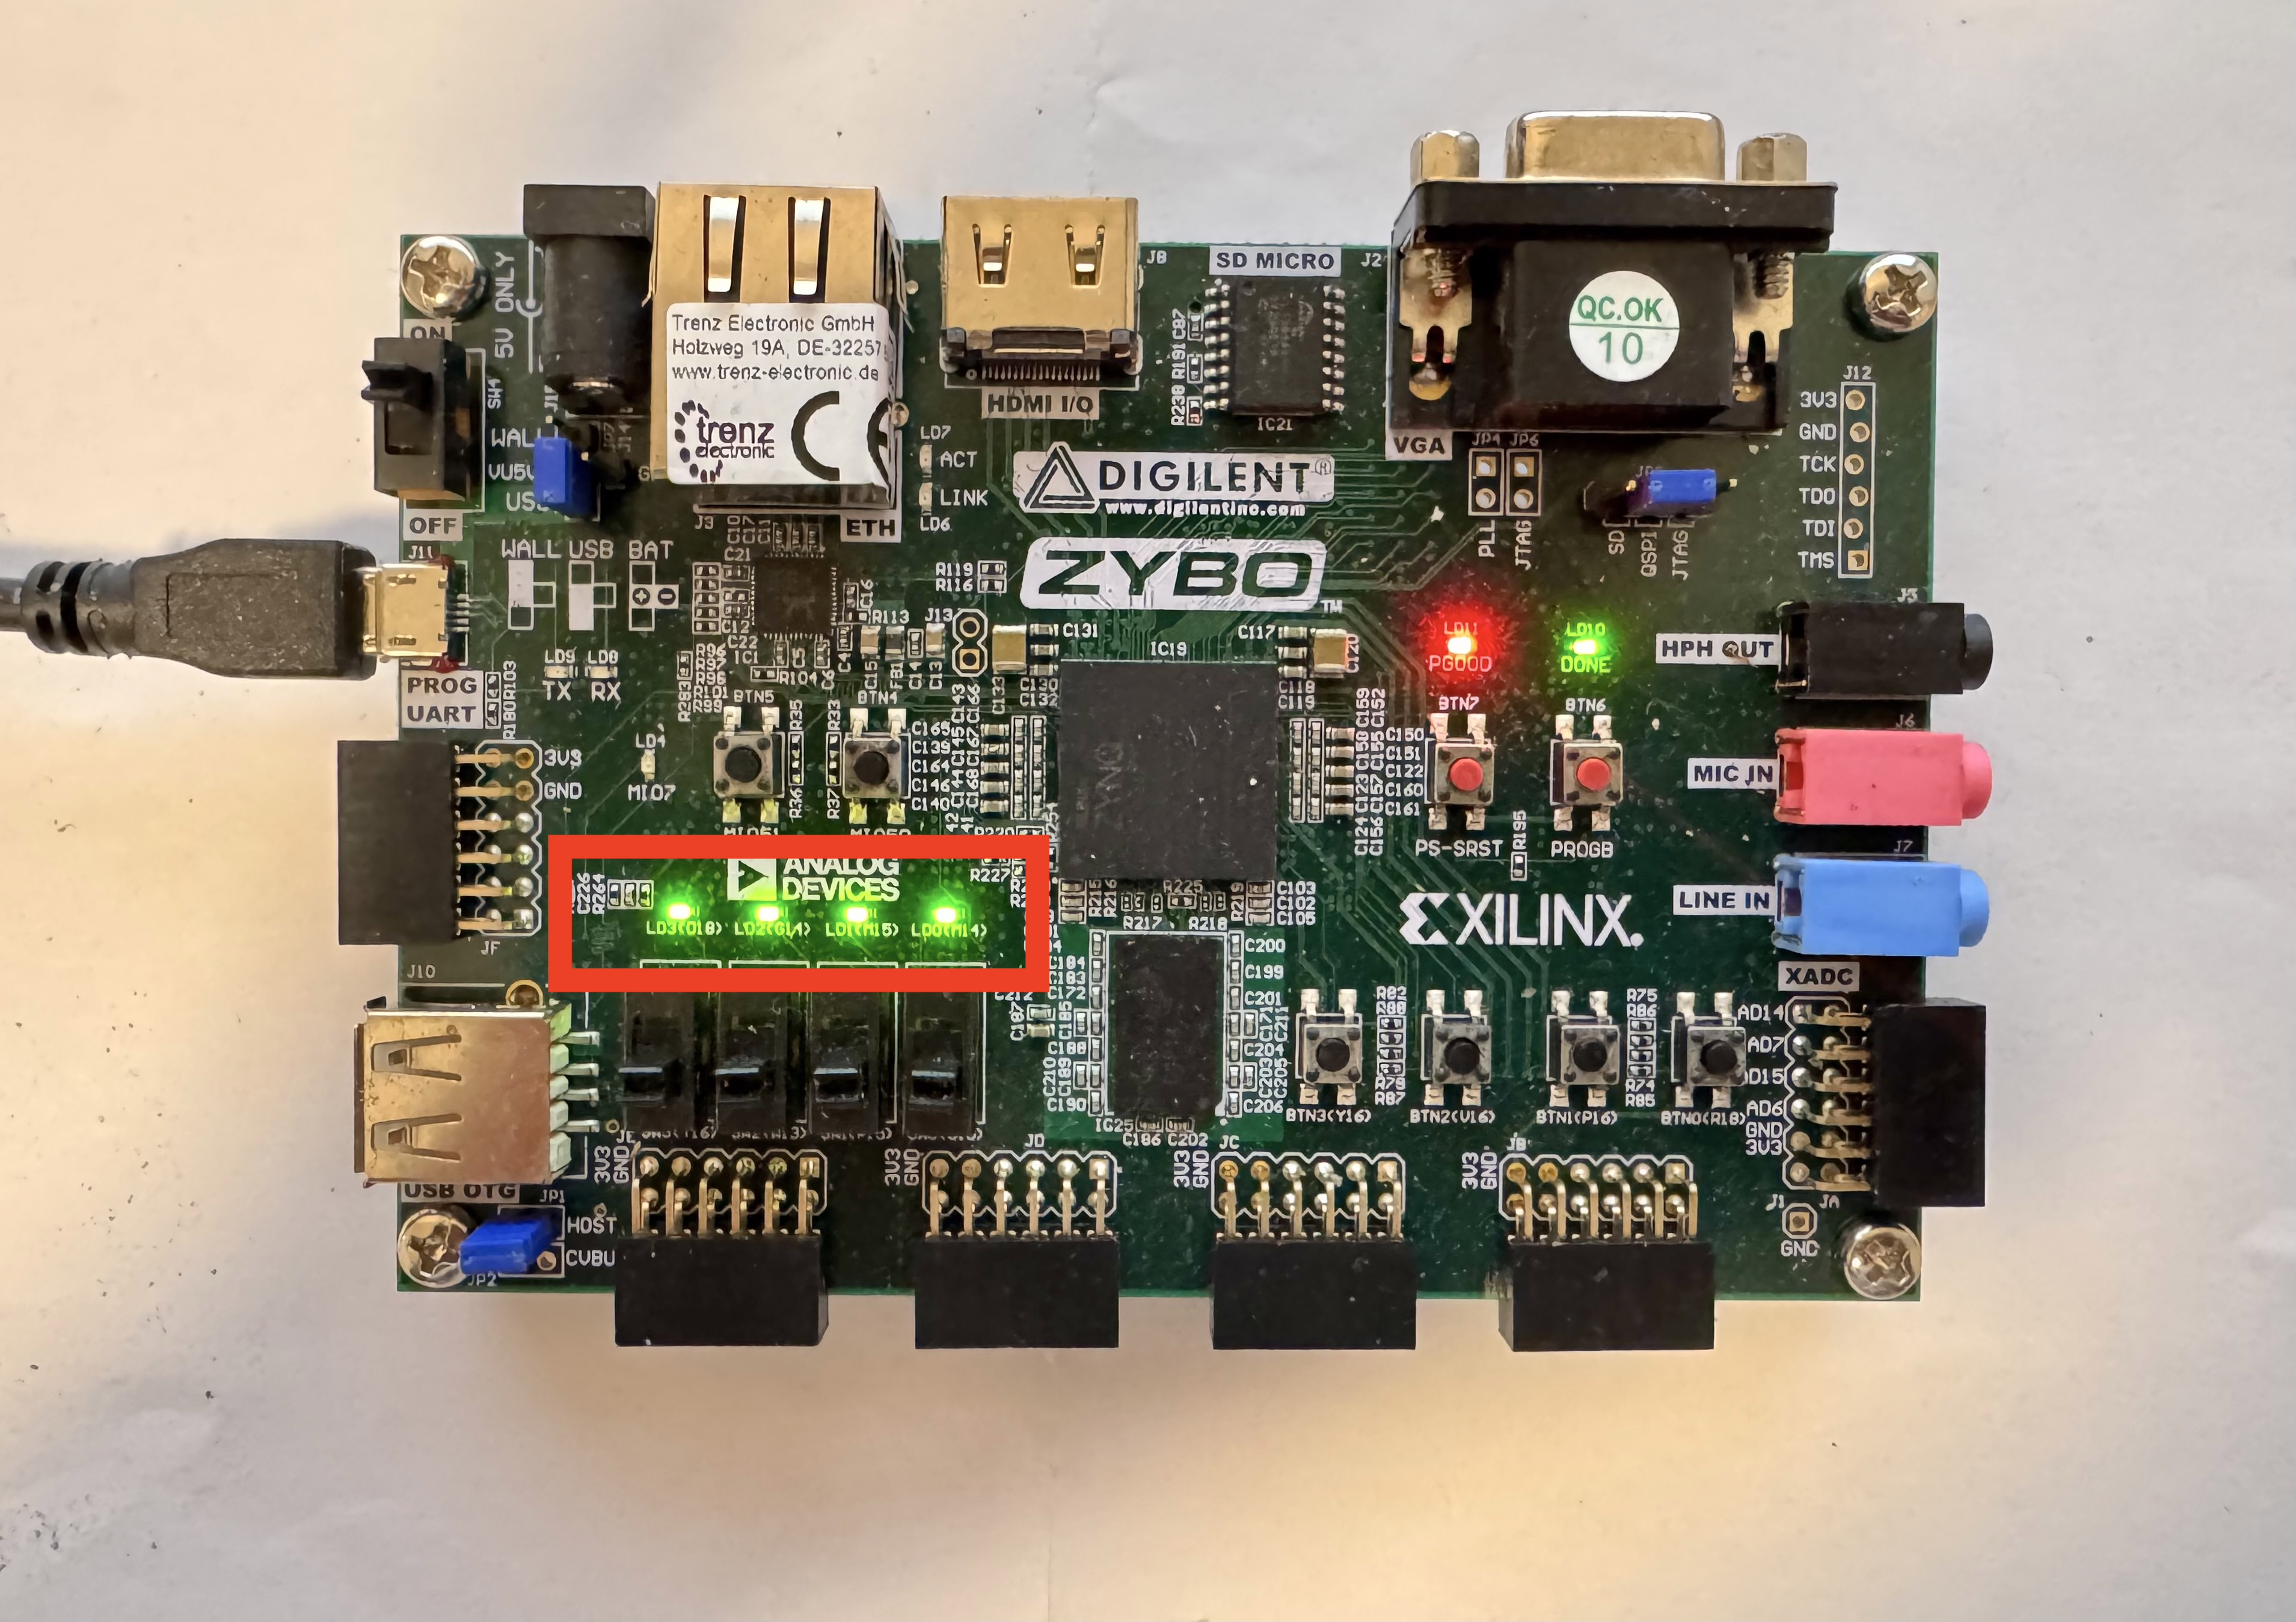
\includegraphics[width=0.9\textwidth]{rwu_output4.jpeg}
  \caption{FPGA hardware output on the Zybo board showing all four LEDs ON (\texttt{GPIO = 0x0F}).}
  \label{fig:fpga-output}
\end{figure}

\subsection{Discussion}
The consistent results between simulation and hardware confirm the following:
\begin{enumerate}
  \item The RWU-RV64I GCC toolchain correctly compiles conditional and arithmetic expressions.
  \item The simulation model matches the physical FPGA implementation at the signal level.
  \item The optimization level \texttt{-O2} preserves program logic and I/O semantics.
\end{enumerate}

This demonstrates that the entire development flow—from compilation to FPGA execution—is stable and reliable for both debugging and optimized builds.  
The LED output serves as a practical visual indicator of the internal program logic, allowing straightforward verification of instruction correctness without requiring serial I/O or additional peripherals.

\section{Summary}
This chapter presented an experimental study of compiler optimization effects on the RWU-RV64I toolchain.  
Different GCC optimization levels were applied to representative C programs to observe their impact on code size, execution behaviour, and simulation results.  
The analysis showed that optimized builds (\texttt{-O2} and above) consistently produced smaller binaries and reliable outputs, while unoptimized builds (\texttt{-O0}) often failed due to missing helper routines and increased instruction count.

A conditional arithmetic and branching program was then used to verify the correct functional behaviour of the optimized binary in both simulation and hardware.  
The results demonstrated identical GPIO outputs in XSIM and on the Zybo FPGA board, confirming that the RWU-RV64I processor and toolchain operate correctly and consistently across environments.  
These findings validate that the applied compiler optimizations preserve program logic and observable I/O behaviour, ensuring reliable execution and efficient code generation for the RWU-RV64I development workflow.

